\documentclass[a4paper,12pt]{article}
\usepackage[top = 2.5cm, bottom = 2.5cm, left = 2.5cm, right = 2.5cm]{geometry}
% Unfortunately, LaTeX has a hard time interpreting German Umlaute. The following two lines and packages should help. If it doesn't work for you please let me know.
\usepackage[T1]{fontenc}
\usepackage[utf8]{inputenc}
% The following two packages - multirow and booktabs - are needed to create nice looking tables.
\usepackage{multirow} % Multirow is for tables with multiple rows within one cell.
\usepackage{booktabs} % For even nicer tables.
% As we usually want to include some plots (.pdf files) we need a package for that.
\usepackage{graphicx}
\usepackage{tikz}
% The default setting of LaTeX is to indent new paragraphs. This is useful for articles. But not really nice for homework problem sets. The following command sets the indent to 0.
\usepackage[spanish]{babel}
\usepackage{setspace}
\setlength{\parindent}{0in}
% Package to place figures where you want them.
\usepackage{float}
% The fancyhdr package let's us create nice headers.
\usepackage{fancyhdr}
\usepackage{amsmath}
\usepackage{amssymb}
\usepackage{natbib}
\usepackage{apalike}
\usepackage{graphicx}
\usepackage{subcaption}
\usepackage{booktabs}
\usepackage{etoolbox}
\usepackage{amsthm}
\AtBeginEnvironment{align}{\setcounter{equation}{0}}
\newenvironment{solution}
  {\renewcommand\qedsymbol{$\blacksquare$}\begin{proof}[Solución]}
  {\end{proof}}
\pagestyle{fancy}

\fancyhf{}

\lhead{\footnotesize Tarea 4}
\rhead{\footnotesize  Rompich}
\cfoot{\footnotesize \thepage}



\begin{document}
    \thispagestyle{empty} % This command disables the header on the first page.

    \begin{tabular}{p{15.5cm}} % This is a simple tabular environment to align your text nicely
    \begin{tabbing}
    Universidad del Valle de Guatemala 
    \\
    Departamento de Matemática\\ Licenciatura en Matemática Aplicada \\ Fecha de entrega: 5 de marzo de 2021  \\
    Rudik R. Rompich   - Carné: 19857\\
    \end{tabbing}
    Estadística 2 - Eugenio Aristondo \\
    \hline % \hline produces horizontal lines.
    \\
    \end{tabular} % Our tabular environment ends here.
    \vspace*{0.3cm} % Now we want to add some vertical space in between the line and our title.
    \begin{center} % Everything within the center environment is centered.
    {\Large \bf Tarea 4
} % <---- Don't forget to put in the right number
        \vspace{2mm}
    \end{center}
    \vspace{0.4cm}

\section{Capítulo 13}
\subsection{Problema 28}
En un experimento factorial con dos niveles para el factor A y tres niveles para el factor B se obtuvieron los datos siguientes.
\begin{center}
    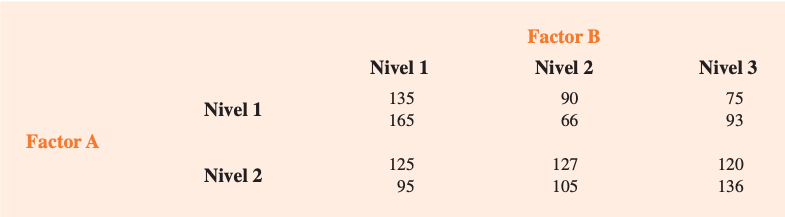
\includegraphics[scale=0.5]{Images/28.png}
\end{center}
Realice una prueba para determinar si hay algunos efectos principales significativos y algún efecto de interacción. Use $\alpha=$  0.05.
\begin{solution}
Comenzamos sacando los promedios de las columnas y filas: 
\begin{center}
    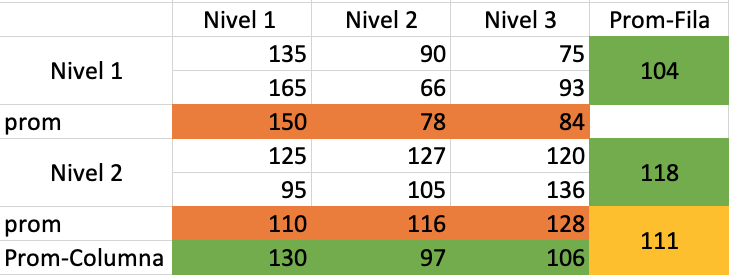
\includegraphics[scale=0.5]{Images/28-tabla.png}
\end{center}
Además, tenemos lo siguiente: 
$$STC=SCA+SCB+SCAB+SCE$$
También contamos con los siguientes parámetros: \begin{itemize}
    \item $a$ = número de niveles del factor A
    \item $b$ = número de niveles del factor B 
    \item $r$ = número de replicaciones
    \item $n_T$ = número total de observaciones realizadas en el experimento; $n_T= abr$
    \item $x_{i j k}=$ observación correspondiente a la $k$ -ésima réplica tomada del tratamiento $i$ del factor A y del tratamiento $j$ del factor $\mathrm{B}$.
    \item  $\bar{x}_{i} .=$ media muestral de las observaciones en el tratamiento $i$ (factor $\mathrm{A}$ )
    \item $\bar{x}_{\cdot j}=$ media muestral de las observaciones en el tratamiento $j$ (factor B)
    \item $\bar{x}_{i j}=$ media muestral de las observaciones correspondientes a la combinación del tratamiento $i$ (factor A) y el tratamiento $j$ (factor B)
    \item $\overline{\bar{x}}=$ media muestral general de todas las $n_{T}$ observaciones
\end{itemize}
Ahora bien, empezamos a calcular: \newline\newline
Paso 1. Calcular la suma total de cuadrados.
\begin{align}
    \mathrm{STC} &=\sum_{i=1}^{a} \sum_{j=1}^{b} \sum_{k=1}^{r}\left(x_{i j k}-\overline{\bar{x}}\right)^{2}\\
    &= \sum_{i=1}^{2} \sum_{j=1}^{3} \sum_{k=1}^{2}\left(x_{i j k}-111\right)^{2}\\
    &=9028
\end{align}
Paso 2. Calcular la suma de cuadrados del factor A.
\begin{align}
\mathrm{SCA}&=\operatorname{br} \sum_{i=1}^{a}\left(\bar{x}_{i} \cdot-\overline{\bar{x}}\right)^{2}\\
            &=(3)(2) \sum_{i=1}^{2}\left(\bar{x}_{i} \cdot-111\right)^{2}\\
            &= 588 
\end{align}
Paso 3. Calcular la suma de cuadrados del factor B.
\begin{align}
\mathrm{SCB}&=\operatorname{ar} \sum_{j=1}^{b}\left(\bar{x}_{\cdot j}-\overline{\bar{x}}\right)^{2}\\
            &= (2)(2)\sum_{j=1}^{3}\left(\bar{x}_{\cdot j}-111\right)^{2}\\
            &= 2328
\end{align}
Paso 4. Calcular la suma de cuadrados debido a la interacción.
\begin{align}
\mathrm{SCAB}&=r \sum_{i=1}^{a} \sum_{j=1}^{b}\left(\bar{x}_{i j}-\bar{x}_{i}-\bar{x}_{\cdot j}+\overline{\bar{x}}\right)^{2}\\
 &= 2 \sum_{i=1}^{2} \sum_{j=1}^{3}\left(\bar{x}_{i j}-\bar{x}_{i}-\bar{x}_{\cdot j}+111\right)^{2}\\
 &= 4392
\end{align}
Paso 5. Calcular la suma de cuadrados debido al error.
\begin{align}
\mathrm{SCE}&=\mathrm{STC}-\mathrm{SCA}-\mathrm{SCB}-\mathrm{SCAB}\\
            &= 9028-588-2328-4392\\
            &= 1720
\end{align}
Por lo tanto, usando la Tabla 13.11, tenemos:
\begin{center}
    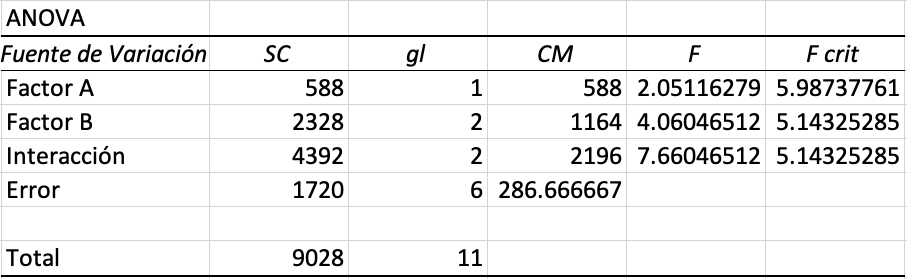
\includegraphics[scale=0.5]{Images/28-ANOVA.png}
\end{center}
\begin{itemize}
    \item Factor A: F=2.0511 y $F_\alpha$= 5,9873
    \item Factor B: F=4,0604 y $F_\alpha$= 5,1432
    \item Interacción: F=7,6604 y $F_\alpha$= 5,1432
\end{itemize}
Es decir que por la prueba F con $\alpha=0.05$, los factores A y B no tienen ningún efecto significativo; mientras que los efectos por interacción sí son significativos ($F>F_\alpha$).
\end{solution}
\subsection{Problema 29}
De los cálculos de un experimento factorial con cuatro niveles para el factor A, tres niveles para el factor B y tres replicaciones se obtuvieron los datos siguientes: STC = 280, SCA = 26, SCB = 23 y SCAB = 175. Establezca la tabla ANOVA y pruebe si hay algunos efectos principales significativos y algún efecto de interacción. Use $\alpha=$ 0.05.
\begin{solution}
Comenzamos encontrando el SCE: 
$$\text{SCE}=\text{STC-SCA-SCB-SCAB}=280-26-23-175=56$$
Considerando la Tabla 13.11 del libro de texto: \begin{center}
    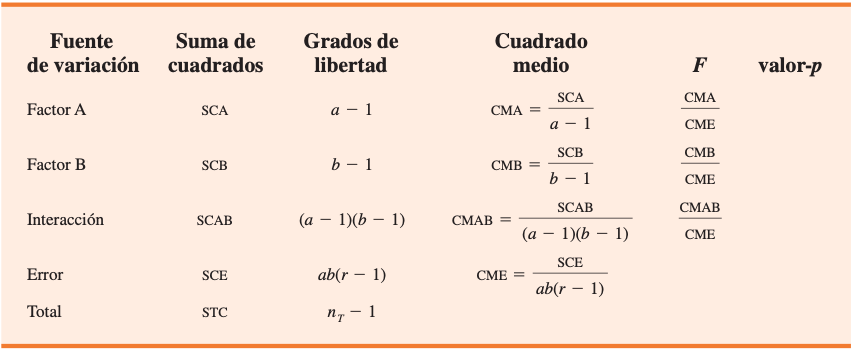
\includegraphics[scale=0.4]{Images/28-tabla-2.png}
\end{center}
Grados de libertad ($a=4$, $b=3$ y $r=3$): 
\begin{enumerate}
    \item $a-1=3$
    \item $b-1=2$
    \item $(a-1)(b-1)=6$
    \item $ab(r-1)=24$
    \item $n_T-1=36-1=35$
\end{enumerate}
Cuadrado medio ( STC = 280, SCA = 26, SCB = 23 y SCAB = 175,SCE=56):
\begin{enumerate}
    \item $CMA=\frac{SCA}{a-1}=\frac{26}{3}=8,667$
    \item $CMB=\frac{SCB}{b-1}=\frac{23}{2}=11,5$
    \item $CMAB= \frac{SCAB}{(a-1)(b-1)}=\frac{175}{6}=29,167$
    \item $CME=\frac{SCE}{ab(r-1)}=\frac{56}{24}=2,333$
\end{enumerate}
Valores F: 
\begin{enumerate}
    \item $\frac{CMA}{CME}=\frac{8,667}{2,333}=3,715$
    \item $\frac{CMB}{CME}=\frac{11,5}{2,333}=4,929$
    \item $\frac{CMAB}{CME}=\frac{29,167}{2,333}=12,502$

\end{enumerate}
   
Los $F_\alpha$: 
\begin{center}
    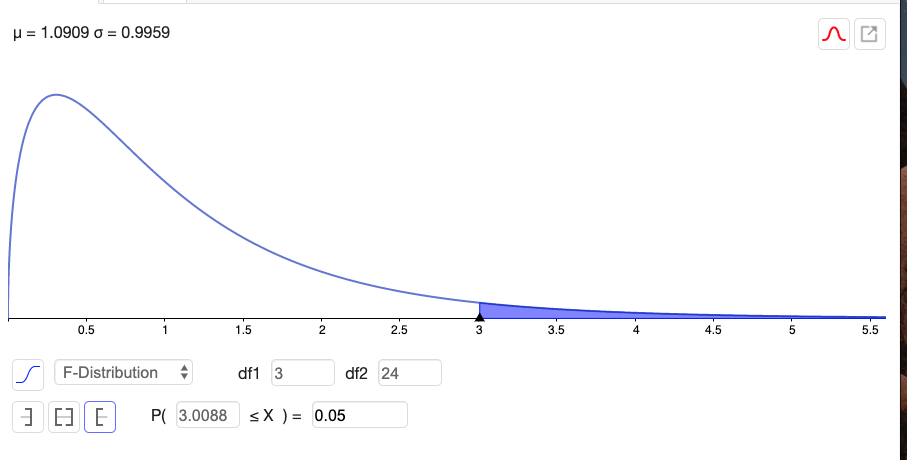
\includegraphics[scale=0.3]{Images/1.png}
\end{center}
\begin{center}
    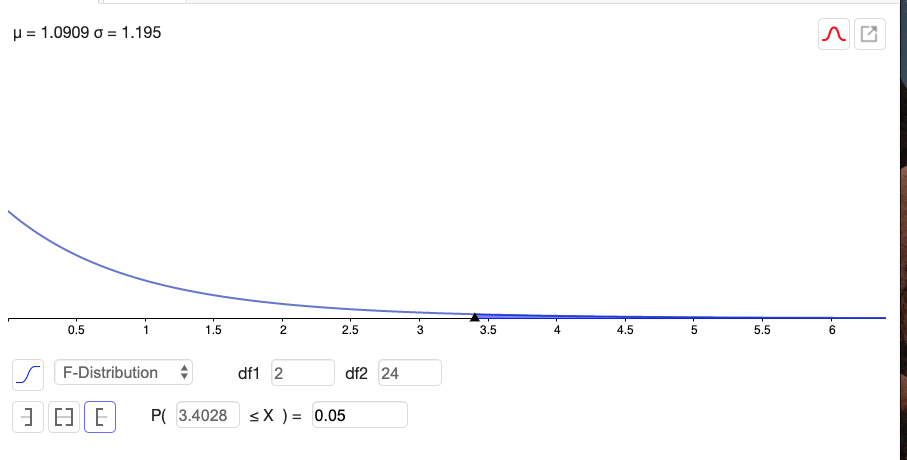
\includegraphics[scale=0.3]{Images/2.png}
\end{center}
\begin{center}
    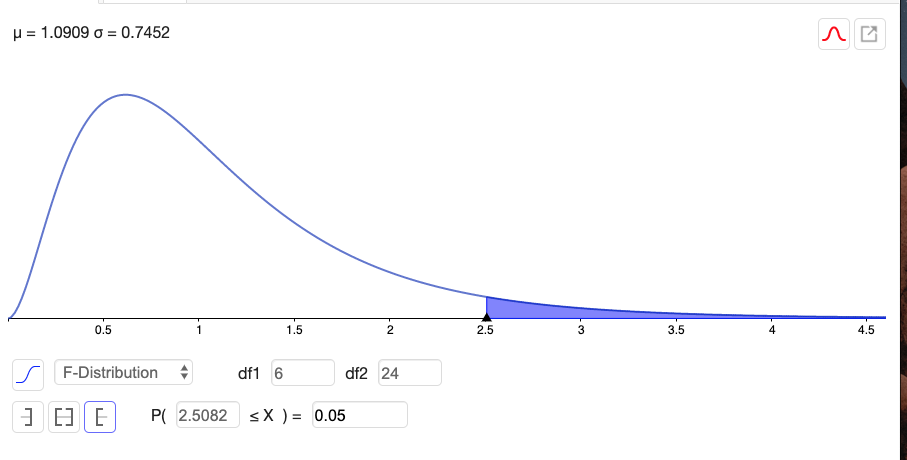
\includegraphics[scale=0.3]{Images/3.png}
\end{center}

Finalmente, tenemos: 
\begin{center}
    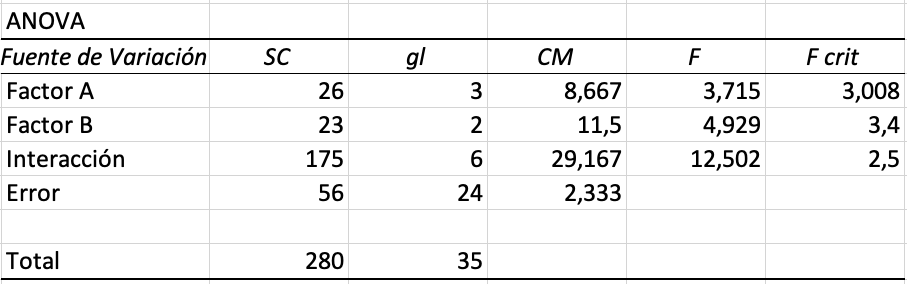
\includegraphics[scale=0.3]{Images/anova.png}
\end{center}
Por lo tanto, se puede afirmar por la prueba F que: 
\begin{enumerate}
    \item Factor A: $F=3.715$ y $F_\alpha=3.007$. Hay evidencia que existe una diferencia significativa.
    \item Factor B: $F=4.929$ y $F_\alpha=3.4$. Hay evidencia que existe una diferencia significativa.
    \item Interacción : $F=12,502$ y $F_\alpha=2.5$. Hay evidencia que existe una diferencia significativa.
\end{enumerate}
\end{solution}
\subsection{Problema 30}
Una empresa de ventas por catálogo realizó un experimento factorial para probar el efecto del tamaño de un anuncio de revista y su diseño sobre el número de solicitudes de catálogos recibido (datos en miles). Se pusieron a consideración tres diseños publicitarios y dos tamaños. Los datos obtenidos se presentan a continuación. Utilice el procedimiento ANOVA para un diseño factorial a fin de probar si hay efectos significativos debido al tipo de diseño, al tamaño del anuncio o a la interacción. Use $\alpha=$ 0.05.
\begin{center}
    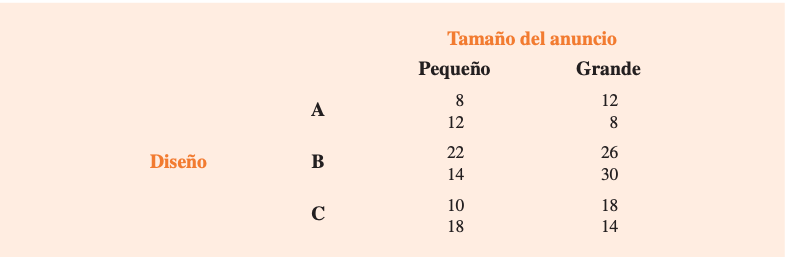
\includegraphics[scale=0.5]{Images/30.png}
\end{center}

\begin{solution}
Haciendo el análisis por medio de Excel, tenemos: 
\begin{center}
    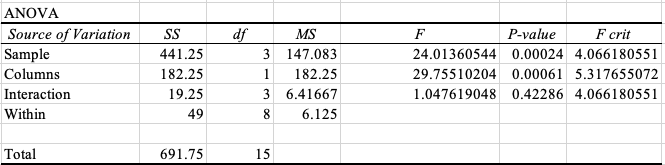
\includegraphics[scale=0.5]{Images/30-bueno.png}
\end{center}
En donde, por la prueba F, se concluye: 
\begin{enumerate}
    \item Diseños; F=24,01360 y $F_\alpha=4,0661$. Existe evidencia suficiente para afirmar que hay efectos significativos.
    \item Tamaño; F=29,7551 y $F_\alpha=5,3176$. Existe evidencia suficiente para afirmar que hay efectos significativos.
    \item Interacción; F=1,047 y $F_\alpha=4,0661$. No existe evidencia de que hayan efectos significativos.
\end{enumerate}
\end{solution}
\subsection{Problema 31}
Un parque de diversión estudió algunos métodos para reducir el tiempo de espera (en minutos) al bajar y subir a los pasajeros a los juegos. Se propusieron dos métodos para realizar estas ta- reas. Para tomar en cuenta las diferencias potenciales debido al tipo de juego y a la interacción que puede haber entre tipo de juego y método de subir y bajar a los pasajeros, se diseñó un ex- perimento factorial. Use los datos siguientes para pobrar cualquier efecto significativo debido al método de subir y bajar a los pasajeros, el tipo de juego y la interacción. Use $\alpha=$ 0.05.
\begin{center}
    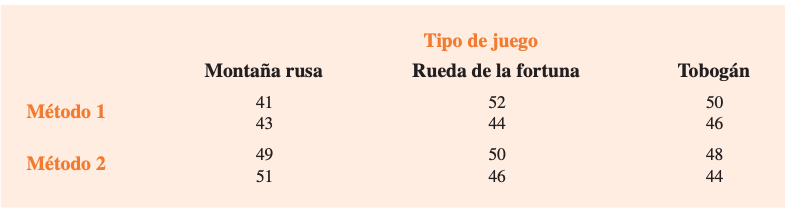
\includegraphics[scale=0.5]{Images/31.png}
\end{center}
\begin{solution}
Considerando el análisis de Excel, tenemos: 
\begin{center}
    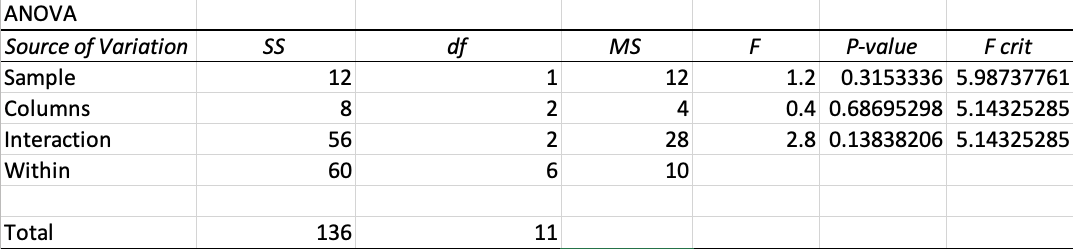
\includegraphics[scale=0.3]{Images/32-anova.png}
\end{center}
A partir de la prueba F, podemos concluir: 
\begin{enumerate}
    \item Métodos: $F=1,2$ y $F_\alpha=5,9873$. No existe evidencia de que hayan efectos significativos.
    \item Tipo de juego: $F=0,4$ y $F_\alpha=5,1432$. No existe evidencia de que hayan efectos significativos.
    \item Interacción: $F=2,8$ y $F_\alpha=5,14325$. No existe evidencia de que hayan efectos significativos.
\end{enumerate}
\end{solution}
\subsection{Problema 32}
En un estudio diseñado para comparar vehículos híbridos (Hybrid) y convencionales (Con- ventional) con equipo similar, Consumer Reports probó varias clases de automóviles híbridos, automóviles a gasolina y vehículos utilitarios deportivos (SUV). Los datos siguientes muestran la clasificación en millas por galón que Consumer Reports obtuvo para dos automóviles com- pactos (Small Car) híbridos, dos automóviles medianos (Midsize Car) híbridos, dos SUV compactos (Small SUV) híbridos y dos SUV medianos (Midsize SUV) híbridos; también se mues- tra el rendimiento en millas por galón obtenidas de ocho modelos convencionales con equipo similar (Consumer Reports, octubre de 2008). Make/Model indica fabricante y modelo; Class (clase), Type (tipo) y MPG (millas por galón).
\begin{center}
    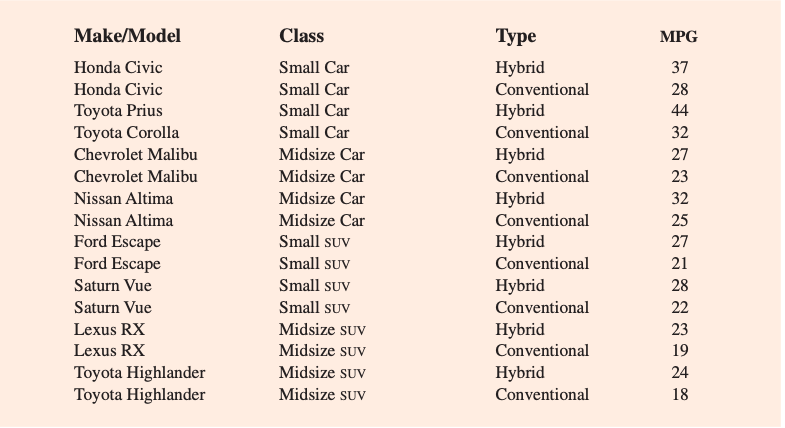
\includegraphics[scale=0.5]{Images/32.png}
\end{center}
Realice pruebas para encontrar efectos significativos debido a la clase, tipo e interacción con un nivel de significancia $\alpha=$ 0.05.
\begin{solution}
Se procederá a tabular los datos:
\begin{center}
    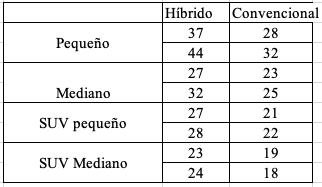
\includegraphics[scale=0.5]{Images/data-last.png}
\end{center}
Con el análisis de Excel tenemos: 
\begin{center}
    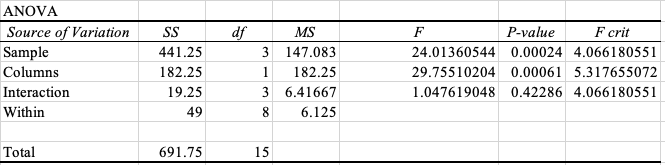
\includegraphics[scale=0.5]{Images/32-bueno.png}
\end{center}
Por medio de la prueba F, concluimos: 
\begin{enumerate}
    \item Clases; F= 24,013 y $F_\alpha=4.0661$. Hay suficiente evidencia para afirmar que existe una diferencia signficativa.
    \item Tipos ; F= 29.7552 y $F_\alpha=5,3176$. Hay suficiente evidencia para afirmar que existe una diferencia signficativa.
    \item Interacción; F=F=1.04761 y $F_\alpha=4,0661$. No hay evidencia de que exista una diferencia.
\end{enumerate}
\end{solution}
\end{document}